\documentclass{article}
\usepackage[utf8]{inputenc}
\usepackage{amsmath, amsthm, amssymb, amsfonts}
\usepackage{tikz}



\title{Homework 5}
\author{DUMA Yehor (31209504)}
\date{11/18}
\begin{document}

\maketitle

\section{Exercise 3}
\textbf{a)}$A =\{1,2,3,4\}$\\ \\
$R_1 = \{\langle 1,1 \rangle, \langle 2,1 \rangle, \langle 3,4 \rangle, \langle 2,2 \rangle, \langle 3,3 \rangle, \langle 4,4\rangle,\langle 4,1 \rangle\}$ \\
$R_2 = \{\langle 3,4 \rangle, \langle 1,2 \rangle, \langle 1,4 \rangle, \langle 2,3 \rangle, \langle 2,4 \rangle, \langle 1,3\rangle\}$ \\
$R_3 = \{\langle 2,4 \rangle, \langle 3,1 \rangle, \langle 3,4 \rangle, \langle 2,2 \rangle, \langle 1,3 \rangle, \langle 4,3\rangle,\langle 4,2 \rangle\}$ \\
$R_4 = \{\langle 1,1 \rangle, \langle 2,4 \rangle, \langle 1,3 \rangle, \langle 2,2 \rangle, \langle 3,1 \rangle, \langle 4,4\rangle , \langle 3,3\rangle, \langle 4,2\rangle\}$ \\ \\
$R_1$ is reflexive, anti-symmetric, nontransitive, nonconnected \\
$R_2$ is irreflexive, asymmetric,transitive, connected \\
$R_3$ is nonreflexive, symmetric nontransitive, nonconnected \\
$R_4$ is \textbf{reflexive, symmetric, transitive}, nonconnected \\ \\
By the preservation of properties all of the inverses $R^{-1}_{1}$-$R^{-1}_{4}$ \textbf{have the same properties} as $R_1$-$R_4$ ($R_1$-$R_4 \neq \varnothing$) \\ \\ 
By definition of complement $R^{'}_{n} \equiv (A \times A) - R_n$, therefore \\ \\ 
$A \times A = \{ \\ \langle 1,1 \rangle, \langle 1,2 \rangle, \langle 1,3 \rangle, \langle 1,4 \rangle, \\ \langle 2,1 \rangle, \langle 2,2\rangle,\langle 2,3 \rangle , \langle 2,4 \rangle, \\ \langle 3,1 \rangle, \langle 3,2 \rangle, \langle 3,3 \rangle, \langle 3,4 \rangle, \\ \langle 4,1 \rangle,\langle 4,2 \rangle,\langle 4,3 \rangle,\langle 4,4 \rangle \}$ \\ \\ 
$R^{'}_{1} = \{\langle 1,2 \rangle, \langle 1,3 \rangle, \langle 1,4 \rangle, \langle 2,3 \rangle, \langle 2,4 \rangle, \langle 3,1\rangle,\langle 3,2 \rangle,\langle 4,2 \rangle,\langle 4,3 \rangle\}$ \\ \\
$R^{'}_{2} = \{\langle 1,1 \rangle, \langle 2,1 \rangle,\langle 2,2 \rangle,\langle 3,1 \rangle,\langle 3,2 \rangle, \langle 3,3 \rangle, \langle 4,1 \rangle, \langle 4,2 \rangle, \langle 4,3 \rangle, \langle 4,4\rangle\}$ \\ \\
$R^{'}_{3} = \{\langle 1,1 \rangle,\langle 1,2 \rangle,\langle 1,4 \rangle, \langle 2,1 \rangle, \langle 2,3 \rangle, \langle 3,2 \rangle, \langle 3,3 \rangle, \langle 4,1\rangle,\langle 4,4 \rangle\}$ \\ \\
$R^{'}_{4} = \{\langle 1,2 \rangle, \langle 1,4 \rangle, \langle 2,1 \rangle, \langle 2,3 \rangle, \langle 3,2 \rangle, \langle 3,4\rangle , \langle 4,1\rangle, \langle 4,3\rangle\}$ \\ \\ \\ 
$R^{'}_{1}$ is irreflexive, nonsymmetric, nontransitive, nonconnected \\ \\
$R^{'}_{2}$ is reflexive, anti-symmetric,transitive, connected \\ \\
$R^{'}_{3}$ is nonreflexive, symmetric nontransitive, nonconnected \\ \\
$R^{'}_{4}$ irreflexive, symmetric, intransitive, nonconnected \\ \\
Equivalence relations are, by definition, reflexive, symmetric, and transitive. Therefore $R_4$ and $R^{-1}_{4}$ are \textbf{equivalence relations}. \\
The partition that is induced on $A$ is $\{\{1,3\},\{2,4\}\}$  \\ \\ 
\textbf{b)} Given the partition $P = \{\{1\}, \{2,3\}, \{4\}\}$ the equivalence relation (must be reflexive, symmetric, and transitive) is \\ \\ 
$R_P = \{\langle 1,1 \rangle, \langle 2,2 \rangle, \langle 3,3 \rangle, \langle 4,4 \rangle, \langle 2,3 \rangle, \langle 3,2\rangle\} $ \\ 

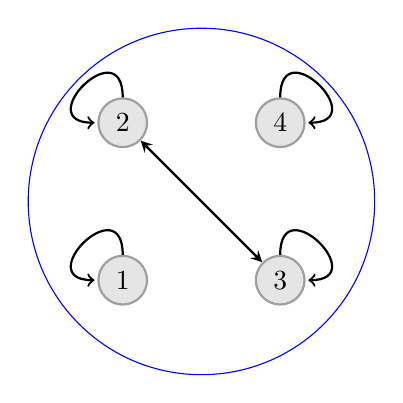
\begin{tikzpicture}[node distance=2cm]
\tikzstyle{place}=[circle,thick,draw=gray!75,fill=gray!20,minimum size=6mm]
\begin{scope}
\draw[color=blue] (0,0) circle [radius=2.2]; 
\node[place] (A) at (-1, -1) {1};
\node[place] (B) at (-1, 1) {2};
\node[place] (C) at (1, -1) {3};
\node[place] (D) at (1, 1) {4};


\draw [thick, stealth-stealth] (B) -- (C);
\draw[thick,->,shorten >=1pt] (A) to [out=90,in=180,loop,looseness=4.8] (A);
\draw[thick,->,shorten >=1pt] (B) to [out=90,in=180,loop,looseness=4.8] (B);
\draw[thick,->,shorten >=1pt] (C) to [out=90,in=0,loop,looseness=4.8] (C);
\draw[thick,->,shorten >=1pt] (D) to [out=90,in=0,loop,looseness=4.8] (D);

\end{scope}
\end{tikzpicture}
\\ \\
\textbf{c)} There are \textbf{15} ways to partition \textbf{4} elements of $A$ into cells of size \textbf{1} to \textbf{4}:
\\

\begin{gather*} 
\binom{4}{4} + \binom{4}{3} + \binom{4}{2} + \binom{4}{1} = 1+4+6+4 = 15
\end{gather*}
\end{document}